\documentclass[10pt,a4paper]{article}
\usepackage[utf8]{inputenc}
\usepackage{titlesec}
\usepackage{amsfonts}
\usepackage{graphicx}
\usepackage{hyperref}
\usepackage{amsmath}
\usepackage{amssymb}
\usepackage{multicol}
\usepackage{multirow}
\usepackage{array}
\usepackage{color}
\usepackage{float}
\usepackage[left=2.50cm, right=2.50cm, top=2.50cm, bottom=2.50cm]{geometry}
\usepackage[txtcentered=true, height=40pt, width=70pt]{thumbs}
\usepackage[german]{babel}
\usepackage[linewidth=1pt]{mdframed}
\usepackage{subfigure}
\usepackage[justification=centering]{caption}
\author{Florian Euchner, Stefan Köbel, Chong Shen, Jan Frederik Dick}

\newcommand{\fancythumb}[2]{
	\addthumb{#1}{\large\sffamily\textbf{\space\space#1\vspace{5pt}}}{white}{#2}
}

\newcommand{\fancyformula}[2]{
	\small
	\raggedright\sffamily\textbf{#1}
	#2
}

\newcommand{\ftransform}{
	~\xrightarrow{~\mathcal{F}~}~
}

\DeclareMathOperator{\sinc}{sinc}
\DeclareMathOperator{\sgn}{sgn}
\DeclareMathOperator{\rect}{rect}
\renewcommand{\Re}{\operatorname{Re}}
\renewcommand{\Im}{\operatorname{Im}}

\pagenumbering{arabic}
\titleformat*{\section}{\sffamily\Large\bfseries}
\titleformat*{\subsection}{\sffamily\large\bfseries}
\titleformat*{\subsubsection}{\sffamily\normalsize\bfseries}

\begin{document}
\section*{Klassifikation von Signale und Systeme}
\fancythumb{Klass.}{teal}
\subsection*{Signal}
Ein Signal ist eine \textbf{Funktion} $x(t)$. Sie liefert für jedes Funktionsargument $t$ einen Funktionswert $x(t)$.
\subsection*{Klassifikation von Signalen}
\begin{tabular}{r p{12cm}}
	\textbf{gerade/ungerade} & $x(t)=x_g(t)+x_u(t)$\\
	 & es gilt: $x_g(-t)=x_g(t)$ und $x_u(-t)=-x_u(t)$, $x_u(0)=0$\\
	 & damit: $x_g(t)=\frac{1}{2}(x(t)+x(-t))$ und $x_u(t)=\frac{1}{2}(x(t)-x(-t))$\\
	 \textbf{reell/imaginär/komplex} & $x(t)=x_r(t)+jx_i(t)$ und $x^*(t)=x_r(t)-jx_i(t)$\\
	 & es gilt: $x_r(t)$ und $x_i(t) \in \mathbb R$\\
	 & damit: $x_r(t)=\frac{1}{2}(x(t)+x^*(t))$ und $x_i(t)=\frac{1}{2j}(x(t)-x^*(t))$\\
	 \textbf{periodisch} & es existiert $T$, sodass $x(t+T)=x(t)$ für alle $t$\\
	 & kleinstes $T$ heißt Periode\\
	 \textbf{einkanalig} & 1 Funktionswerk, z.B. $x(t)$\\
	 \textbf{mehrkanalig} & mehrere Funktionswerte, z.B.
	$\begin{bmatrix}
		x_1(t) \\ 
		x_2(t)
	\end{bmatrix}$\\
	\textbf{eindimensional} & 1 Funktionsargument, z.B. $x(t)$\\
	\textbf{mehrdimensional} & mehrere Funktionsargumente, z.B. $x(t,x,y)$\\
	\textbf{zeitkontinuierlich} & zeitkontinuierliches Funktionsargument, $x(t)$ mit $t \in \mathbb R$\\
	\textbf{zeitdiskret} & zeitdiskretes Funktionsargument, $x(n)$ mit $n \in \mathbb Z$\\
	\textbf{wertkontinuierlich} & kontinuierlicher Funktionswert\\
	\textbf{wertdiskret} & diskreter Funktionswert\\
	\textbf{analog} & zeitkontinuierliche und wertkontinuierlich\\
	\textbf{digital} & zeitdiskret und wertdiskret\\
\end{tabular}

\subsection*{Zeitkontinuierliche Signale}
\begin{tabular}{r >{\centering\arraybackslash} p{7cm} l}
	\textbf{Sprungfunktion} & $u(t)=\begin{cases}
	1 & \text{für } t>0\\
	0 & \text{für } t<0\\
	\end{cases}$ & \raisebox{-.5\height}{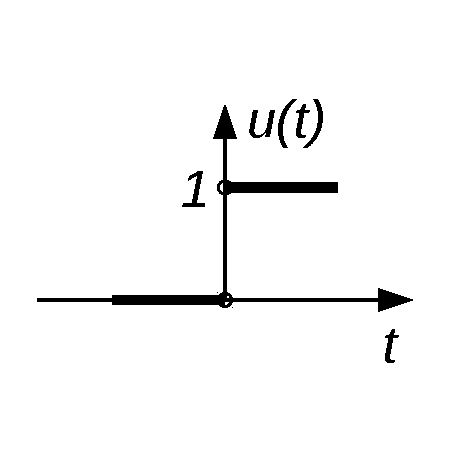
\includegraphics[width=3cm]{img/zeitkontSprungfunktion}} \\

	\textbf{Vorzeichenfunktion} &
	{$\!\begin{aligned}
		 \sgn(t) &= \begin{cases}
			1 & \text{für } t>0\\
			-1 & \text{für } t<0\\
		\end{cases} \\
		&= 2 ~ u(t) - 1
	\end{aligned}$}
	& \raisebox{-.5\height}{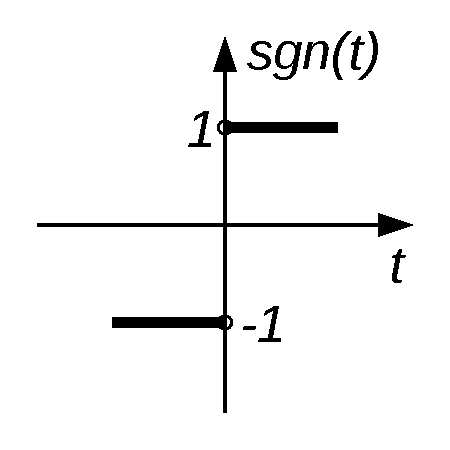
\includegraphics[width=3cm]{img/zeitkontVorzeichenfunktion}} \\ 

	\textbf{Rechteckfunktion} &
	{$\!\begin{aligned}
		 \rect(t) &= \begin{cases}
			1 & \text{für } |t| < 1\\
			0 & \text{für } |t| > 1\\
		\end{cases} \\
		&= u(t - 1) - u(t + 1)
	\end{aligned}$}
	& \raisebox{-.5\height}{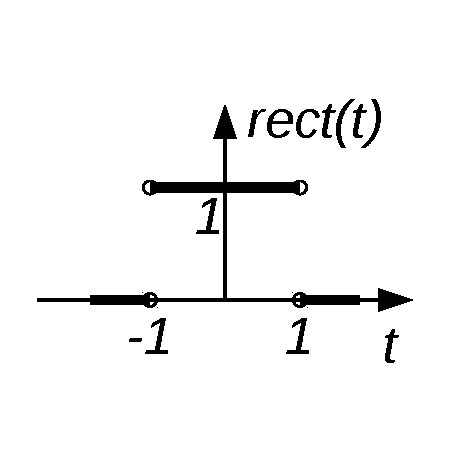
\includegraphics[width=3cm]{img/zeitkontRechteckfunktion}} \\

	\textbf{o-Funktion} & $o(x) = \begin{cases}
		0 & \text{für } t = 0\\
		1 & \text{für } t \neq 0\\
	\end{cases}$ \\

	\textbf{verschob. Rechteck} & $A ~ \rect \left(\dfrac{t-\dfrac{t_1+t_2}{2}}{\dfrac{t_2-t_1}{2}} \right)$ & \raisebox{-.5\height}{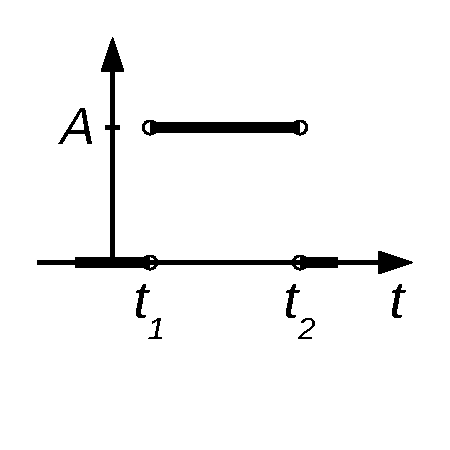
\includegraphics[width=3cm]{img/zeitkontVerschobenesRechteck}} \\

	\textbf{Dreieck} & $A ~ \dfrac{t}{T} ~ \rect \left(\dfrac{t-\frac{T}{2}}{\dfrac{T}{2}} \right)$ & \raisebox{-.5\height}{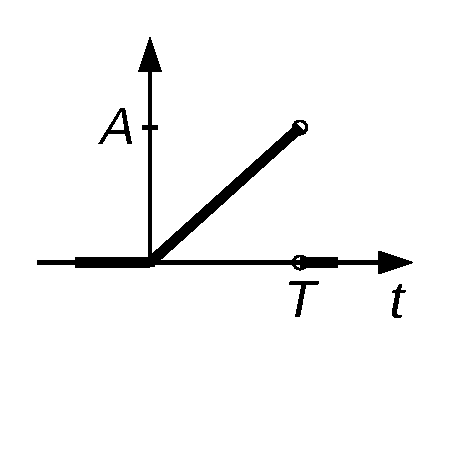
\includegraphics[width=3cm]{img/zeitkontDreieck}} \\

	\textbf{Impulsantwort} & $h(t) = T(\delta(t))$ \\
	\textbf{Sprungantwort} & $a(t) = T(a(t))$
\end{tabular}

\subsection*{Zeitdiskrete Signale}
\begin{tabular}{r >{\centering\arraybackslash} p{7cm} l}
	\textbf{Sprungfunktion} & $u(n)=\begin{cases}
	1 & \text{für } n \geq 1\\
	0 & \text{für } n < 1\\
	\end{cases}$ & \raisebox{-.5\height}{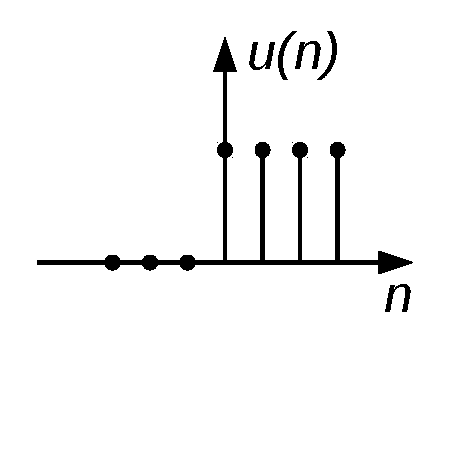
\includegraphics[width=3cm]{img/zeitdiskSprungfunktion}} \\

	\textbf{Impulsfunktion} &
	{$\!\begin{aligned}
		 \delta(t) &= \begin{cases}
			1 & \text{für } n = 0 \\
			0 & \text{für } n \neq 0 \\
		\end{cases} \\
		&= u(t - 1) - u(t + 1)
	\end{aligned}$}
	 & \raisebox{-.5\height}{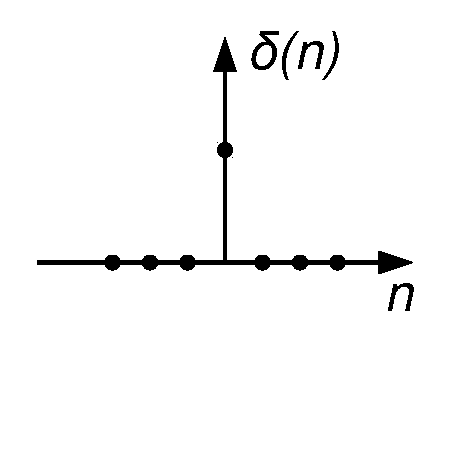
\includegraphics[width=3cm]{img/zeitdiskImpulsfunktion}} \\
	
	\textbf{Rechteckfunktion} &
	{$\!\begin{aligned}
		\rect \left(\dfrac{n}{N} \right) &= \begin{cases}
			1 & \text{für } |n| \leq N\\
			0 & \text{für } |n| > N\\
		\end{cases} \\
		&= u(n + N) - u(n - N - 1)
	\end{aligned}$} & \raisebox{-.5\height}{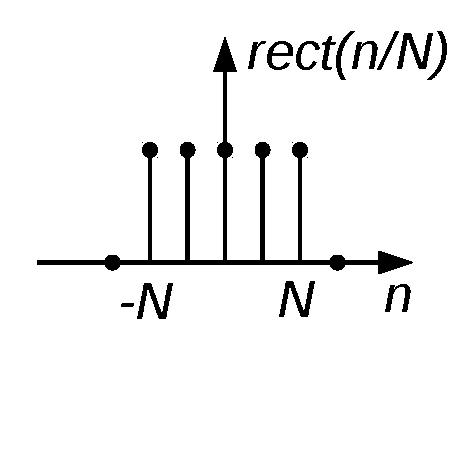
\includegraphics[width=3cm]{img/zeitdiskRechteckfunktion}} \\
	
	\textbf{Impulsantwort} & $h(n) = T(\delta(n))$ \\
	\textbf{Sprungantwort} & $a(n) = T(a(n))$ \\
\end{tabular} 

\subsection*{System}
	Das System hat einen \textbf{Operator}, der eine Funktion auf eine andere Funktion abbildet. Ein System heißt \textbf{zeitkontinuierlich, zeitdiskret, analog, digital}, wenn alle beteiligten Signale so heißen.
\subsection*{Klassifikation von Systemen}
Sei $a \in \mathbb R, a > 0$.
\vspace{.5em}

\begin{centering}
\begin{tabular}{r | r | p{11.5cm}}
	\textbf{Gedächtnis} &
	\textbf{gedächtnislos} & $y(t)$ hängt \textbf{nur} vom momentanem $x(t)$ ab \\
	& \textbf{mit Gedächtnis} & $y(t)$ hängt auch von zukünftigen $x(t + a)$ oder vergangenen $x(t - a)$ ab \\

	\textbf{Kausalität} &
	\textbf{kausal} & $y(t)$ hängt von vergangenen $x(t - a)$ und momentanem $x(t)$ ab \\
	& \textbf{antikausal} & $y(t)$ hängt von zukünftigen $x(t + a)$ und momentanem $x(t)$ ab \\
	& \textbf{nichtkausal} & $y(t)$ hängt von zukünftigen $x(t + a)$, aber nicht von momentanem $x(t)$ ab \\

	\textbf{Zeitinvarianz} &
	\textbf{zeitinvariant} & $y(t) = T(x(t)) \implies y(t-\tau)=T(x(t-\tau))$, d.h.
	Systemverhalten unabhängig von Alter des Systems \\
	& \textbf{zeitvariant} & Systemverhalten abhängig von Alter des Systems\\

	\textbf{Linearität} &
	\textbf{linear} & Superpositionsprinzip gilt, d.h.
	\textbf{Homogenität} $T(ax(t)) = a ~ T(x(t))$ und
	\textbf{Additivität} $T \left(\sum x_i(t) \right) = \sum T(x_i(t)$ sind erfüllt. Dies impliziert $T(0) = 0$. \\
	& \textbf{nichtlinear} & Bedingungen treffen nicht zu \\

	\textbf{Stabilität} &
	\textbf{BIBO-stabil} & $\vert x(t)\vert\leq M_x <\infty \implies \vert y(t)\vert\leq M_y < \infty ~ \forall t, x(t)$, "Beschränktes Eingangssignal $\implies$ beschränktes Ausgangssignal." \\
	& \textbf{instabil} & für beschränktes Eingangssignal ist unbeschränktes Ausgangssignal möglich
\end{tabular}
\end{centering}

\begin{figure}[H]
	\centering
	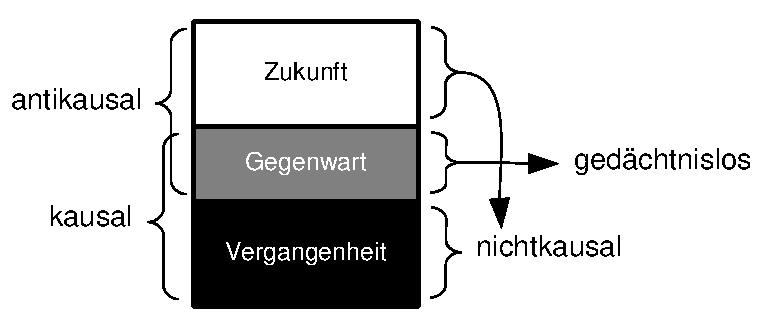
\includegraphics[width=8cm]{img/ZeiteigenschaftenVonSystemen}
\end{figure}

\subsection*{Parallel- und Kettenschaltung von Systemen}
\begin{itemize}
	\item \textbf{Parallelschaltung} $y(t)=T_1(x(t))+T_2(x(t))+...+T_N(x(t))$
	\item \textbf{Kettenschaltung} 	$y(t)=T_N(...T_2(T_1(x(t)))...)$
\end{itemize}

\newpage


\section*{Impulsantwort und Faltung}
\fancythumb{Faltung}{red}
\subsection*{Impulsantwort und Sprungantwort}
\begin{tabular}{l l}
	\textbf{Impulsantwort} & Antwort $h(t)$ eines Systems auf die Anregung mit einer Dirac-Funktion $\delta(t)$ \\
	\textbf{Sprungantwort} & Antwort $a(t)$ eines Systems auf die Anregung mit einer Sprungfunktion $u(t)$ \\
\end{tabular}
\subsubsection*{Überprüfung von Systemeigenschaften mit $h(t)$}
\begin{tabular}{l p{12cm}}
	\textbf{E1)} & System gedächtnislos $\Longleftrightarrow y(t) = c~x(t)$\\ & $\rightarrow$ keine Ableitungen $\frac{d}{dt}x(t)$ dürfen auftreten \[h(t)=c~\delta(t)\]\\
	\textbf{E2)} & System kausal $\Longleftrightarrow h(t)=0 \quad \forall t<0$ bzw.\\ & \[y(t)=\int_{-\infty}^{\infty}h(\tau)x(t-\tau)d\tau=\int_{0}^{\infty}h(\tau)x(t-\tau)d\tau\] $\rightarrow$ nur in Vergangenheit, weil $\tau$ positiv.
	\[=\int_{-\infty}^{t}x(\tau)h(t-\tau)d\tau\] \\
	\textbf{E3)} & System BIBO-Stabil $\Longleftrightarrow \int_{-\infty}^{\infty}|h(t)|dt<\infty \quad \substack{\nleftarrow\\[-1em] \rightarrow}\quad h(t)\overset{t\rightarrow\infty}{\longrightarrow}0$
\end{tabular}
\subsection*{Faltung}
\subsubsection*{Grafische Faltung}
\begin{figure}[H]
	\centering
	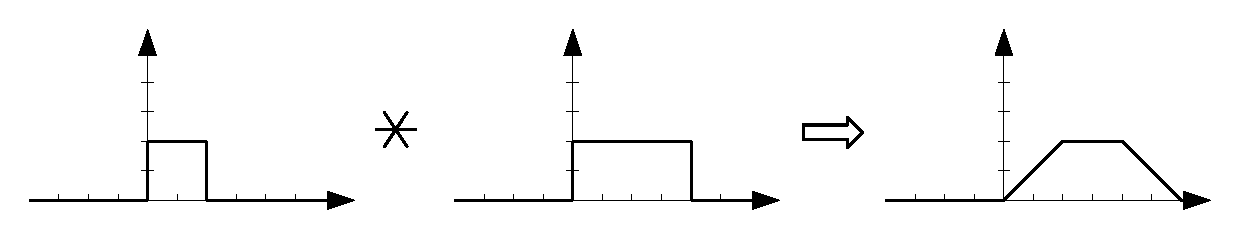
\includegraphics[width=0.75\textwidth]{img/faltung1.pdf}
	\caption*{Faltung zweier Rechtecksignale}
\end{figure}
\begin{figure}[H]
	\centering
	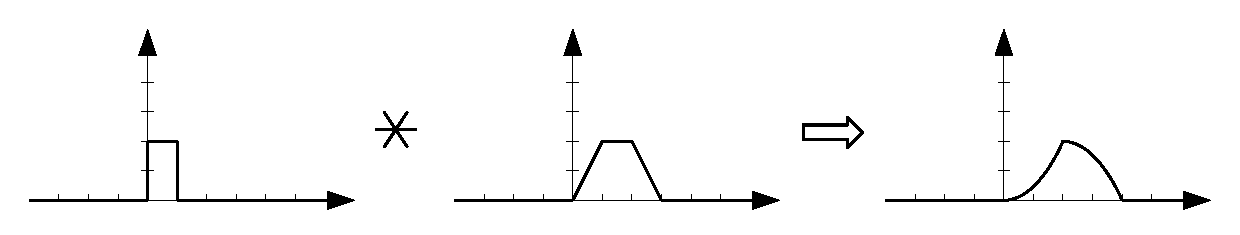
\includegraphics[width=0.75\textwidth]{img/faltung2.pdf}
	\caption*{Faltung eines Rechtecks mit einem Signal mit zwei linearen Flanken}
\end{figure}
\begin{figure}[H]
	\centering
	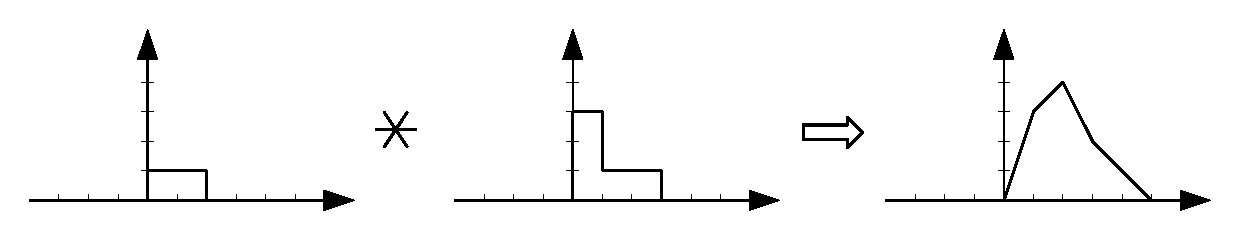
\includegraphics[width=0.75\textwidth]{img/faltung3.pdf}
	\caption*{Faltung verschieden hoher Rechtecksignale}
\end{figure}
\subsubsection*{Analytische Faltung}
\subsubsection*{Definition}
\[ (f \ast g)(t)=\int_\mathbb{R}f(\tau)\cdot g(t-\tau) d\tau \]
Das Ausgangssignal $y(t)$ eines Systems ist das Eingangssignal $x(t)$ mit der Impulsantwort $h(t)$ gefaltet.
\[ y(t) = (x \ast h)(t)=\int_\mathbb{R}x(\tau)\cdot h(t-\tau) d\tau\]
\subsubsection*{Eigenschaften}
\begin{tabular}{l l p{12cm}}
	\textbf{E1)}&\textbf{Kommutativ} & $(x \ast h)(t) = (h \ast x)(t)$\\
	\textbf{E2)}&\textbf{Assoziativ}(Kettenschaltung) & $((x \ast h_1) \ast h_2)(t) = (x \ast (h_1 \ast h_2))(t)$\\
	\textbf{E3)}&\textbf{Distributiv}(Parallelschaltung) & $((x \ast h_1)(t)+(x \ast h_2)(t) = (x \ast (h_1 + h_2))(t)$
\end{tabular}
\begin{center}
	\centering
\begin{tabular}{l | c | c | c |}
& \textbf{E4)}&\textbf{E5)}&\textbf{E6)}\\
\hline
Wenn $x(t)$ & $=0, \quad \forall t<0$ & Dauer $D_x$ & verschoben um $\tau_x$\\
und $h(t)$ & $=0, \quad \forall t<0$ & Dauer $D_h$ & verschoben um $\tau_h$\\
dann $y(t)$ & $=0, \quad \forall t<0$ & Dauer $D_x+D_h$ & verschoben um $\tau_x+\tau_h$\\
\end{tabular}
\end{center}
\newpage


\section*{DGLn}
\fancythumb{DGL}{magenta}
\subsection*{Lineare Differenzengleichungen mit konstanten Koeffizienten}
\begin{tabular}{r p{12cm}}
	\textbf{DGL} & $\alpha(D) ~ y(n) = \beta(D) ~ x(n)$, wobei $D^k(y) = y(n-k)$ und $\alpha$, $\beta$ Polynome vom Grad N bzw. M \\
	\textbf{Eingangssignal} & $x(n) = u(n) ~ A ~ q^n$ \\
	\textbf{Anfangswerte} & $y(-1)$, …, $y(-N)$ und (wenn nicht aus $x(n)$ ersichtlich) $x(-1)$, …, $x(-M)$ \\
	\textbf{Lösung} & Funktion $y(n)$ für $n \geq 0$, die DGL für Eingangssignal erfüllt. $y(n)$ muss nicht die Anfangsbedingungen erfüllen, da $n \geq 0$
\end{tabular}

\subsubsection*{Homogene Lösung $y_h$}
Bestimme $y_h(n)$, sodass $\alpha(D) ~ y_h(n) = 0 ~ \forall n \in \mathbb Z$. Bestimme alle $\tilde N$ verschiedene Nullstellen $z_1$, …, $z_{\tilde N}$ der Gleichung $\alpha(z^{-1}) = 0$ nach durchmultiplizieren mit $z^N$.

\paragraph{Nullstellen verschieden:} Jede Nullstelle ist einfach $\Leftrightarrow \tilde N = N$
\[
	y_h(n) = c_1 ~ z_1^n + … + c_N ~ z_N^n
\]

\paragraph{Mehrfache Nullstellen:} $z_1$ ist $k$-fache Nullstelle $\implies \tilde N = N - k < N$
\[
	y_h(n) = \left(c_{1,1} + c_{1,2} ~ n + … + c_{1,k} ~ n^{k-1}\right) ~ z_1^n + c_2 ~ z_2^n + … + c_{\tilde N} ~ z_{\tilde N}^n
\]

\subsubsection*{Partikuläre Lösung $y_p$}
Bestimme ein $y_p(n)$ so, dass $\alpha(D) ~ y_p(n) = \beta(D) ~ x(n) ~ \forall n \geq 0$ für ein spezifisches $x(n) = u(n) ~ A ~ q^n, n \geq 0$.

\paragraph{q keine Nullstelle von $\alpha \Leftrightarrow q \neq z_i ~ \forall i$}
\[
	y_p(n) = A ~ \frac{\beta(q^{-1})}{\alpha(q^{-1})} ~ q^n
\]
\paragraph{q ist k-fache Nullstelle von $\alpha \Leftrightarrow \exists i: ~ q = z_i$} Mit $\alpha^{(k)}(D)$ ist k-te Ableitung von $\alpha(D)$:
\[
	y_p(n) = A ~ \frac{\beta(q^{-1})}{\alpha^{(k)}(q^{-1})} (-q ~ n)^k ~ q^n
\]

\subsubsection*{Allgemeine Lösung $y$ und Lösung mit Anfangswerten}
\[
	y(n) = y_h(n) + y_p(n)
\]
Um die Anfangswerte zu berücksichtigen, müssen Koeffizienten $c_1, …, c_N$ bzw. $c_{1,0}, …, c_{1,k}, …, c_{\tilde N}$ bestimmt werden. Setze dazu Werte von $x(n)$ und $y(n)$ in Abhängigkeit der Koeffizienten in die DGL für $n = 0, …, N - 1$ ein und Löse LGS.

\vspace{.5em}
\raggedright
\textbf{Warnung:} \textit{Nicht} die Koeffizienten durch Lösen von $y(-1) = y(n)$ für $n = -1$ etc. bestimmen - das wird falsch, denn $y(n)$ ist für $n < 0$ keine Lösung, da $y_p$ dann keine Lösung!

\subsubsection*{Impulsantwort $h$}
Für Anfangsbedingungen gilt $y(-1) = … = y(-N) = 0$.
\paragraph{Für $N > M$:} Es ist klar, dass $\alpha(D) ~ y_h(n) = 0 ~ \forall n \in \mathbb Z$ für beliebige Koeffizienten $c$. Nun wird das System mit der Impulsfunktion 
\[
	\delta(n) =
	\begin{cases}
		1 & \textnormal{für } n = 0 \\
		0 & \textnormal{sonst}
	\end{cases}
\]
angeregt. Für $n > M$ ist die Differenzengleichung also homogen, da auf der rechten Seite $x(n) = \delta(n)$ höchstens in der $M$-ten Verzögerung $D^M ~ x(n) = \delta(n - M) = 0$ steht.

\vspace{.5em}
Ansatz: Impulsantwort $h(n) = y(n) = u(n) ~ y_h(n)$ stimmt schon für $n > M$, bestimmte Koeffizienten so, dass $h(n)$ auch für $n = 0, …, M$ passt. Berechne LGS durch Einsetzen von $y(n)$, $x(n) = \delta(n)$ in DGL für $n = 0, …, N - 1$ mit $N$ Gleichungen und den $N$ unbekannten Koeffizienten $c$.

\[
	h(n) = u(n) ~ y_h(n) ~~ \textnormal{…mit den durch LGS bestimmten Koeffizienten $c$}
\]

\paragraph{Sonst:} Setze Eingangssignal $x(n) = u(n) ~ A ~ q^n$ zu $A = q = 1$, sodass $x(n) = u(n)$. Bestimme allgemeine Lösung der DGL mit diesem Eingangssignal, Lösung ist Sprungantwort $a(n) = y(n)$.

\vspace{.5em}
Da gilt $\delta(n) = u(n) - u(n - 1)$ folgt aus Linearität mit Systemoperator $T$ und $T(\delta(n)) = T(u(n) - u(n - 1))$:
\[
	h(n) = a(n) - a(n-1)
\]

\newpage
\section*{Fourierreihe zeitkontinuierlicher Signale}
\fancythumb{FR}{blue}
\subsection*{Definition}
\[
	x(t) = \sum_{k=-\infty}^\infty c_k ~ e^{jk\Omega t} = a_0 + \sum_{k=1}^\infty \left( a_k ~ \cos(k \Omega t) + b_k ~ \sin(k \Omega t) \right)
\]

\begin{centering}
\begin{tabular}{ >{\centering\arraybackslash} m{7cm} >{\centering\arraybackslash} m{1cm} >{\centering\arraybackslash} m{7cm} }

\[
	c_k = \frac{1}{T} ~ \int_T x(t) ~ e^{-jk\Omega t} ~ \mathrm dt
\] & \textit{\sffamily oder} & {
\[
	a_0 = \frac{1}{T} \int_T x(t) ~ \mathrm dt
\]
\[
	a_k = \frac{2}{T} \int_T x(t) ~ \cos(k\Omega t) ~ \mathrm dt, ~ k \in \mathbb Z
\]
\[
	b_k = \frac{2}{T} \int_T x(t) ~ \sin(k\Omega t) ~ \mathrm dt, ~ k \in \mathbb Z
\]
} \\
\end{tabular}
\end{centering}

\subsection*{Eigenschaften}
\begin{multicols}{2}
\fancyformula{Spiegelung}{
	\[ x(-t)  \ftransform c_{-k} \]
}

\fancyformula{Konjugiert komplex}{
	\[ x^*(t)  \ftransform c^*_{-k} \]
}

\fancyformula{Symmetrie}{
 \begin{align*}
	x(t) \textnormal{ gerade reell } &\Longleftrightarrow c_k \textnormal{ gerade reell } \\
	x(t) \textnormal{ gerade imaginär } &\Longleftrightarrow c_k \textnormal{ gerade imaginär } \\
	x(t) \textnormal{ ungerade reell } &\Longleftrightarrow c_k \textnormal{ ungerade imaginär } \\
	x(t) \textnormal{ ungerade imaginär } &\Longleftrightarrow c_k \textnormal{ ungerade reell }
\end{align*}
}

\fancyformula{Linearität}{
	\[ \sum_i \alpha_i ~ x_i(t) \ftransform \sum_i \alpha_i ~ c_{i, k} \]
}

\fancyformula{Verschiebung}{
	\[ x(t - t_0) \ftransform e^{-jk\Omega t_0} ~ c_k \]
	\[ e^{jk_0\Omega t} ~ x(t) \ftransform c_{k-k_0}, ~ k_0 \in \mathbb Z \]
}

\fancyformula{Dehnung}{
	\[ a > 0: x(at) \ftransform c_k \textnormal{ mit Grundfrequenz } a\Omega \]
}

\fancyformula{Differentiation}{
	\[ x^{(n)}(t) \ftransform (jk\Omega)^n ~ c_k \]
}

\fancyformula{Integration}{
	\[ \int_{-\infty}^t x(\tau) ~ \mathrm d\tau \ftransform \frac{1}{jk\Omega} ~ c_k \textnormal{ wenn } c_0 = 0 \]
}

\fancyformula{Moment}{
	\[ \sum_{k=-\infty}^\infty k^n ~ c_k = \frac{1}{(j\Omega)^n} ~ x^{(n)}(t) \bigg|_{t=0} \]
}

\fancyformula{Faltung}{
	\[ \frac{1}{T} \int_T x_1(\tau) ~ x_2(t - \tau) \mathrm ~ d\tau \ftransform c_{1,k} ~ c_{2, k} \]
	\[ x_1(t) ~ x_2(t) \ftransform \sum_{l=-\infty}^{\infty} c_{1, l} ~ c_{2, k - l} \]
}

\fancyformula{Parsevalsche Gleichung}{
	\[ \frac{1}{T} \int_T |x(t)|^2 \mathrm dt = \sum_{k = -\infty}^{\infty} |c_k|^2 = a_0 + \frac{1}{2} \sum_{k=1}^{\infty} \left(|a_k|^2 + |b_k|^2 \right) \]
}
\fancyformula{Anfangswert}{
	\[ x(0) = \sum_{k=-\infty}^{\infty} c_k \]
}
\end{multicols}

\newpage

\section*{Fouriertransformation zeitkontinuierlicher Signale}
\fancythumb{FT}{violet}
\subsection*{Definition}
\begin{multicols}{2}
	\[ X(j\Omega)=\int_{-\infty}^{\infty}x(t)e^{-j\Omega t}dt \]
	\[ x(t)=\int_{-\infty}^{\infty}X(j\Omega)e^{j\Omega t} \frac{d\Omega}{2\pi} \]
\end{multicols}
\subsection*{Eigenschaften}
\begin{multicols}{2}
	
\fancyformula{Spiegelung}{\[ x(-t)\ftransform X(-j\Omega) \]}
\fancyformula{Konjugiert komplex}{\[ x^*(t) \ftransform X^*(-j\Omega)\]}
\fancyformula{Symmetrie}{
\begin{align*}
	x(t) \textnormal{ gerade reell} &\Longleftrightarrow X(j\Omega) \textnormal{ gerade reell} \\
	x(t) \textnormal{ gerade imaginär} &\Longleftrightarrow X(j\Omega) \textnormal{ gerade imaginär} \\
	x(t) \textnormal{ ungerade reell} &\Longleftrightarrow X(j\Omega) \textnormal{ ungerade imaginär} \\
	x(t) \textnormal{ ungerade imaginär} &\Longleftrightarrow X(j\Omega) \textnormal{ ungerade reell} \\
\end{align*}
}
\fancyformula{Dualität / Vertauschbarkeit}{\[ X(jt)\ftransform 2\pi x(-\Omega) \]}
\fancyformula{Linearität}{\[ \sum_{i} a_i x_i(t) \ftransform \sum_{i} a_i X_i(j\Omega)\]}
\fancyformula{Verschiebung}{
\begin{align*}
	x(t-t_0) &\ftransform e^{-j\Omega t_0}X(j\Omega) \\
	e^{j\Omega_0t}x(t) &\ftransform X(j\Omega-j\Omega_0)
\end{align*}
}
\fancyformula{Dehnung}{
\begin{align*}
	x(at) &\ftransform \frac{1}{a}~X\bigg(j\frac{\Omega}{a}\bigg), a>0 \\
	\frac{1}{a}~x\bigg(\frac{t}{a}\bigg) &\ftransform X(ja\Omega), a>0
\end{align*}
}
\fancyformula{Differentiation}{
\begin{align*}
	x^{(n)}(t) &\ftransform (j\Omega)^nX(j\Omega) \\
	(-jt)^nx(t) &\ftransform \frac{\mathrm d^n X(j\Omega)}{\mathrm d\Omega^n}
\end{align*}	
}
\fancyformula{Integration}{
	\[\int_{-\infty}^{t}x(\vartheta)d\vartheta \ftransform \frac{1}{j\Omega} X(j\Omega) o(\Omega)+\pi X(0)\delta(\Omega)\]
	\[\frac{j}{t}x(t)o(t)+\pi x(0) \delta(t)  \ftransform \int_{-\infty}^{\Omega}X(j\sigma)d\sigma \]
}
\fancyformula{Moment}{
\begin{align*}
	\int_{-\infty}^{\infty}t^n x(t)dt &= j^n \frac{d^nX(j\Omega)}{d\Omega^n} \bigg|_{\Omega=0} \\
	\int_{-\infty}^{\infty}\Omega^n X(j\Omega)\frac{d\Omega}{2\pi}&=(-j)^n x^{(n)}(t) \bigg|_{t=0}
\end{align*}	
}
\fancyformula{Faltung}{
\begin{align*}
	(x_1 \ast x_2)(t) &\ftransform X_1(j\Omega)X_2(j\Omega)\\
	x_1(t)x_2(t) &\ftransform \frac{1}{2\pi} (X_1 \ast X_2)(j\Omega)
\end{align*}
}
\fancyformula{Parsevalsche Gleichung}{\[ \int_{-\infty}^{\infty}x_1(t)x_2^*(t)dt=\int_{-\infty}^{\infty}X_1(j\Omega)X_2^*(j\Omega)\frac{d\Omega}{2\pi} \]}
\fancyformula{Anfangswert}{
	\[ X(0)=\int_{-\infty}^{\infty}x(t)dt\qquad x(0)=\int_{-\infty}^{\infty}X(j\Omega)\frac{d\Omega}{2\pi} \]	
}
\end{multicols}
\newpage

\subsection*{Wichtige Fouriertransformationen}
Seien $T>0$, $\Omega_g>0$.
\begin{multicols}{2}
	\small
	\[ \delta(t) \ftransform 1 \]
	\[ \frac{1}{2 \pi} \ftransform \delta(\Omega) \]
	\[ \delta(t - t_0) \ftransform e^{-j\Omega t_0} \]
	\[ \frac{1}{2 \pi} ~ e^{j \Omega_0 t} \ftransform \delta(\Omega - \Omega_0) \]
	\[ \cos(\Omega_0 t) \ftransform \pi \left( \delta(\Omega - \Omega_0) + \delta(\Omega + \Omega_0) \right) \]
	\[ \sin(\Omega_0 t) \ftransform \frac{\pi}{j} \left( \delta(\Omega - \Omega_0) - \delta(\Omega + \Omega_0) \right) \]
	\[ \sgn(t) \ftransform \frac{2}{j \Omega} ~ o(\Omega) \]
	\[ \frac{j}{\pi t} ~ o(t) \ftransform \sgn(t) \]
	\[ u(t) \ftransform \pi \delta(\Omega) + \frac{1}{j \Omega} ~ o(\Omega) \]
	\[ \frac{1}{2} \delta(t) + \frac{j}{2 \pi t} ~ o(t) \ftransform u(\Omega) \]
	\[ \rect \left(\frac{t}{T} \right) \ftransform 2 T ~ \sinc(\Omega T) \]
	\[ \frac{\Omega_g}{\pi} ~ \sinc(\Omega_g t) \ftransform \rect \left( \frac{\Omega}{\Omega_g} \right) \]
	\[ \left(1 - \frac{|t|}{T} \right) ~ \rect \left(\frac{t}{T} \right) \ftransform T ~ \sinc^2 \left( \frac{\Omega T}{2} \right) \]
	\[ e^{-at} ~ u(t) \ftransform \frac{1}{a+j\Omega},\quad \Re(a)>0 \]
	\[ \frac{t^{n-1}}{(n-1)!} ~ e^{-at}u(t) \ftransform \frac{1}{(a+j\Omega)^n},\quad \Re(a)>0 \]
	\[ e^{-a\lvert t \rvert} \ftransform \frac{2a}{a^2+\Omega^2},\quad \Re(a)>0\]
	\[ e^{-a\lvert t \rvert} ~ \sgn(t) \ftransform -j\frac{2\Omega}{a^2+\Omega^2},\quad \Re(a)>0 \]
	\[ e^{-at^2} \ftransform \sqrt{\frac{\pi}{a}}~e^{-\Omega^2/4a},\quad \Re(a)>0 \]
	\[ \cos^2\left(\frac{\pi t}{2T}\right)~\rect\left(\frac{t}{T}\right) \ftransform \frac{\sin(\Omega T)}{\Omega[1-(\Omega T/\pi)^2]} \]
\end{multicols}

\newpage
\section*{Fourierreihe zeitdiskreter Signale}
\fancythumb{DFS}{cyan}
\subsection*{Definition}
\[
	x(n) = \sum_{k = 0}^{N - 1} c_k ~ e^{j \frac{2 \pi n}{N} k} ~ \textnormal{ mit } ~ c_k = \frac{1}{N} ~ \sum_{n = 0}^{N - 1} x(n) ~ e^{-j \frac{2 \pi n}{N} k}
\]

\subsection*{Existenzbedingung}
$x(n)$ muss periodisch sein, was nur für rationale ($\in \mathbb Q$) normierte Frequenzen $f$ der Fall ist, zur Probe Vorfaktor von $n$ so ersetzen, dass Periodizität für rationales $f$ vorliegen würde. Sei beispielsweise
\[
	x(n) = \sin(a ~ x) \stackrel{!}{=} \sin(2\pi f ~ x) \implies f = \frac{a}{2 \pi}
\]
Somit ist $x(n)$ periodisch $\Longleftrightarrow a = \pi ~ q, ~ q \in \mathbb Q$. Da Summe endlich existiert DFS für periodische $x(n)$ immer.

\subsection*{Eigenschaften}
\begin{multicols}{2}
\fancyformula{Periodizität}{
	\[ c_{k + N} = c_k ~ \forall k \in \mathbb N \]
}

\fancyformula{Parseval'sche Gleichung,}{
	\textit{mittlere Leistung von $x(n)$}
	\[ \frac{1}{N} ~ \sum_{n = 0}^{N - 1} |x(n)|^2 = \sum_{k = 0}^{N - 1} |c_k|^2 \]
}
\end{multicols}

\section*{Fouriertransformation zeitdiskreter Signale}
\fancythumb{DTFT}{pink}
\subsection*{Definition}
\[
	x(n) = \int_{2\pi} X\left(e^{j\omega} \right) ~ e^{j\omega n} ~ \frac{\mathrm d\omega}{2 \pi} ~~ \textnormal{mit} ~~ X \left(e^{j\omega} \right) = \sum_{n = -\infty}^{\infty} x(n) ~ e^{-j\omega n}
\]
\subsection*{Eigenschaften}
\begin{multicols}{2}
	
\fancyformula{Spiegelung}{\[ x(-n)\ftransform X \left(e^{-j\omega} \right) \]}
\fancyformula{Konjugiert komplex}{\[ x^*(n) \ftransform X^* \left(e^{-j\omega} \right)\]}
\fancyformula{Symmetrie}{
\begin{align*}
	x(n) \textnormal{ gerade reell} &\Longleftrightarrow X(e^{j\omega}) \textnormal{ gerade reell} \\
	x(n) \textnormal{ gerade imaginär} &\Longleftrightarrow X(e^{j\omega}) \textnormal{ gerade imaginär} \\
	x(n) \textnormal{ ungerade reell} &\Longleftrightarrow X(e^{j\omega}) \textnormal{ ungerade imaginär} \\
	x(n) \textnormal{ ungerade imaginär} &\Longleftrightarrow X(e^{j\omega}) \textnormal{ ungerade reell} \\
\end{align*}
}
\fancyformula{Periodizität}{\textit{Neu!} \[ X \left(e^{j(\omega + 2\pi)}\right) = X(e^{j\omega}) \]}
\fancyformula{Linearität}{\[ \sum_{i} a_i x_i(n) \ftransform \sum_{i} a_i X_i\left(e^{j\omega} \right)\]}
\fancyformula{Verschiebung}{
\begin{align*}
	x(n - n_0) &\ftransform e^{-j\omega n_0} ~ X\left(e^{j\omega} \right) \\
	e^{j\omega_0 n} ~ x(n) &\ftransform X \left(e^{j (\omega - \omega_0)} \right)
\end{align*}
}
\fancyformula{Differentiation}{
\[
	(-jn)^m ~ x(n) \ftransform \frac{\mathrm d^m X(e^{j\omega})}{\mathrm d\omega^m}
\]
}
\fancyformula{Moment}{
\begin{align*}
	\sum_{n=-\infty}^{\infty} n^m ~ x(n) &= j^m \frac{d^m X \left(e^{j\omega} \right)}{d\omega^m} \bigg|_{\omega=0} \\
	x(0) &= \int_{2\pi} X \left(e^{j\omega} \right) ~ \frac{\mathrm d\omega}{2\pi}
\end{align*}	
}
\fancyformula{Faltung}{
\begin{align*}
	(x_1 \ast x_2)(n) &\ftransform X_1 \left(e^{j\omega} \right) ~ X_2 \left(e^{j\omega} \right)\\
	x_1(n) ~ x_2(n) &\ftransform \int_{2\pi} X_1 \left(e^{j\lambda} \right) ~ X_2 \left(e^{j (\omega - \lambda)} \right) ~ \frac{\mathrm d\lambda}{2\pi}
\end{align*}
}
\fancyformula{Parsevalsche Gleichung}{\[ \sum_{n=-\infty}^{\infty}x_1(n) ~ x_2^*(n) = \int_{2 \pi} X_1 \left(e^{j\omega} \right) ~ X_2^* \left(e^{j\omega} \right) ~ \frac{d\omega}{2\pi} \]}
\end{multicols}
\end{document}
